\documentclass[tikz,border=10pt]{standalone}
\usepackage{tikz}
\usepackage{tikz-cd}
\usetikzlibrary{arrows,automata,shapes,positioning,decorations.pathmorphing}
% \tikzset{->,>=stealth',auto}
\tikzset{->,auto}
\tikzset{>={Latex[width=2mm,length=2mm]}}
\tikzset{state/.style={shape=circle, draw, fill=white, initial text=,
    inner sep=.5mm, minimum size=2mm}}
\tikzset{state with output/.style={shape=rectangle split, rectangle
    split parts=2, draw, fill=white,
    initial text=, inner sep=1mm}}
\tikzset{every node={font=\footnotesize}}

\begin{document}
  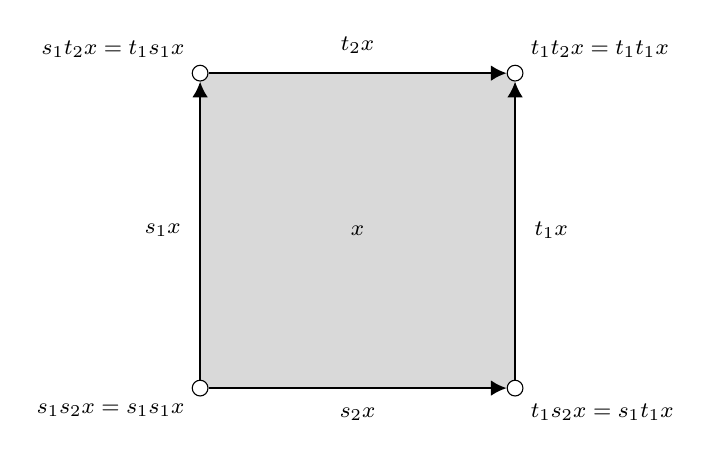
\begin{tikzpicture}[node distance=2cm, align=center]
    \tikzstyle{every node}=[font=\footnotesize]
    \tikzstyle{every state}=[fill=white,shape=circle,inner
    sep=.5mm,minimum size=3mm]
    \path[fill=black!15] (0,0) to (4,0) to (4,4) to (0,4) to (0,0);
    \title{unfolded HDA}
    % face 1
    \node[state] (q01) [label=below left:{$s_1  s_2x = s_1  s_1x$}]                 {};
    \node (q11) [right of=q01, label=below:{$s_2x$}]                                                             {};
    \node (q14) [above of=q01, label=left:{$s_1x$}]                                                              {};
    \node[state] (q03) [right of=q11, label=below right:{$t_1  s_2x = s_1  t_1x$}]  {};
    \node[state] (q02) [above of=q14, label=above left:{$s_1  t_2x = t_1  s_1x$}]   {};
    \node (q12) [above of=q03, label=right:{$t_1x$}]                                                             {};
    \node[state] (q04) [above of=q12, label=above right:{$t_1  t_2x = t_1  t_1x$}]  {};
    \node (q13) [right of=q02, label=above:{$t_2x$}]                                                             {};
    \node (q21) [right of=q14]                                                                                              {$x$};
    
    \draw [->][draw=black, thick] (q01) to node [below] {} (q03);
    \draw [->][draw=black, thick] (q01) to node [left] {} (q02);
    \draw [->][draw=black, thick] (q02) to node [below] {} (q04);
    \draw [->][draw=black, thick] (q03) to node [left] {} (q04);


  \end{tikzpicture}
\end{document}